\documentclass[a4paper,10pt]{scrartcl}
\usepackage[a4paper,left=31.5mm,right=31.5mm,top=30mm,bottom=40mm]{geometry}
\usepackage{float}
\usepackage{fancyhdr}
\usepackage{enumitem}
\usepackage{amsmath,amssymb}
\numberwithin{figure}{section}
\usepackage{tikz}
\usetikzlibrary{shapes.geometric,shapes.arrows,arrows.meta,positioning,calc}
\usepackage[colorlinks=true,linkcolor=blue,linktoc=page]{hyperref}

\setlength{\parindent}{0pt}
\setlength{\parskip}{0.6\baselineskip}
\setlist{topsep=2pt,itemsep=3pt,parsep=0pt}

% ---------- page styles ----------
\pagestyle{fancy}
\fancyhf{}
\renewcommand{\headrulewidth}{0pt}
\fancyfoot[C]{\thepage}
\fancypagestyle{plain}{\fancyhf{}\renewcommand{\headrulewidth}{0pt}\fancyfoot[C]{\thepage}}
\fancypagestyle{tp}{\fancyhf{}\renewcommand{\headrulewidth}{0pt}\fancyfoot[C]{\footnotesize\thepage}}

\newcommand{\code}[1]{\texttt{\renewcommand{\_}{\textunderscore\hspace{0pt}}#1}}

% ---------- TikZ styles ----------
\tikzset{
  ent/.style={ellipse,draw,minimum width=2.7cm,minimum height=1.05cm,font=\sffamily\bfseries\footnotesize,inner sep=1pt,align=center},
  rel/.style={font=\sffamily\footnotesize,text=blue!40!black},
  arr/.style={-{Latex[length=1.6mm]},line width=0.5pt},
  ubox/.style={draw,rounded corners=2pt,minimum width=2.3cm,minimum height=0.65cm,font=\sffamily\scriptsize,align=center,fill=white},
  stp/.style={draw,rounded corners=3pt,minimum width=1.75cm,minimum height=0.9cm,font=\sffamily\scriptsize,align=center,fill=white,inner sep=2pt},
  thead/.style={fill=black,text=white,font=\sffamily\bfseries\scriptsize,minimum height=0.42cm,inner sep=1pt,align=center},
  trow/.style={font=\sffamily\scriptsize,minimum height=0.42cm,inner sep=1pt,align=center},
}

% \dbtable{id}{position}{header}{comma-separated rows}{width}
\newcommand{\dbtable}[5]{%
  \node[thead,minimum width=#5] (#1) at (#2) {#3};%
  \def\prevnode{#1}%
  \foreach \r [count=\i] in {#4}{%
    \ifodd\i \def\rowcol{gray!30}\else\def\rowcol{gray!12}\fi
    \node[trow,minimum width=#5,fill=\rowcol,below=0pt of \prevnode.south] (#1-\i) {\r};%
    \xdef\prevnode{#1-\i}%
  }%
}
% \bigarrow{x0}{y}{length}{half-height}
\newcommand{\bigarrow}[4]{%
  \fill[gray!35] (#1,{#2+0.55*#4}) -- ({#1+#3-0.9},{#2+0.55*#4}) -- ({#1+#3-0.9},{#2+#4}) -- ({#1+#3},#2) -- ({#1+#3-0.9},{#2-#4}) -- ({#1+#3-0.9},{#2-0.55*#4}) -- (#1,{#2-0.55*#4}) -- cycle;%
}

\begin{document}

% ====================== TITLE PAGE ======================
\thispagestyle{tp}
\vspace*{-8mm}
\noindent\rule{1.09\textwidth}{1.6mm}
\vspace{5mm}
\begin{flushright}
{\Huge\bfseries SOFTWARE REQUIREMENTS\\ SPECIFICATION\par}
\vspace{9mm}
{\Huge\bfseries for\par}
\vspace{8mm}
{\Huge\bfseries GATED:\\ APARTMENT TRACKER\par}
\vspace{4mm}
{\large\bfseries A Smart Digital Platform for Apartment and Society Management\par}
\vspace{5mm}
{\Large\bfseries Version 1.0\par}
\vspace{6mm}
{\Large\bfseries Prepared by : 1. Khushi Dangi (1024030101)\\
2. Ridham Sharma  (1024030121)\\
3. Geetika Parakh (1024030115)\\
4. Harnoor Singh (1024030937)\par}
\vspace{1mm}
{\large\bfseries Group 3C14\par}
\vspace{5mm}
{\Large\bfseries Submitted to : Prof. Anushka\par}
\vspace{1mm}
{\large\bfseries UCS503 -- Software Engineering\\
Computer Science and Engineering Department\\
Thapar Institute of Engineering and Technology, Patiala\par}
\vspace{5mm}
{\Large\bfseries October 2026\par}
\vspace{1mm}
{\large\bfseries Mid-Semester Evaluation\par}
\end{flushright}
\newpage

% ====================== CONTENTS ======================
\tableofcontents
\newpage

% ====================== 1 INTRODUCTION ======================
\section{Introduction}
\subsection{Purpose}
In modern residential complexes and gated communities, it is very difficult to maintain society data using physical logbooks, paper receipts, spreadsheets and unorganized messaging groups (e.g.\ WhatsApp). Data can change, get misplaced or become outdated at any moment: new residents move in, visitors enter continuously, maintenance staff changes and complaints get overlooked.

``GATED: Apartment Tracker'' is the solution. It is an official mobile and web-accessible platform engineered to centralize, streamline and secure all residential society workflows. The main concept of ``GATED'' is to eliminate paper-based registers and fragmented communication channels by offering automated role-based access, transparent complaint handling, gate security monitoring, facility booking and centralized administration for modern housing societies.

\subsection{Intended Audience and Reading Suggestions}
This SRS is for developers, system architects, project managers, QA engineers, academic evaluators, society management committee members and testers. Further, the discussion will provide all the internal, external, functional and also non-functional information about ``GATED: Apartment Tracker''.

\begin{itemize}
\item \textbf{Developers and QA Engineers:} Sections 2.3 (Product Functions), 3 (System Features) and 4 (Nonfunctional Requirements).
\item \textbf{System Architects and Evaluators:} Sections 1.3 (Project Scope), 2.1 (Product Perspective) and 2.5 (Design).
\item \textbf{End-Users and Administrators:} Sections 2.2 (User Classes and Characteristics) and 2.5 (Design).
\end{itemize}

\subsection{Project Scope}
``GATED: Apartment Tracker'' creates a space for Residents, Society Administrators, Security Personnel and Maintenance Staff for managing a housing society in one integrated digital ecosystem.

A resident registers, selects the residential society and links his/her specific flat number. After that the resident can submit complaints and maintenance tickets (specifying category, priority and description), monitor the ticket lifecycle in real time, view society notices and submit amenity booking requests.

Society Administrators oversee all society activities. They verify and approve new administrative signups, review unassigned complaints, assign tasks directly to registered maintenance staff by employee ID and broadcast notices.

Security personnel at the society gates log visitor entries and exits, record vehicle details and cross-verify visitor credentials to prevent unauthorized intrusions.

Maintenance employees view the tickets specifically assigned to them by administrators, track the issue details, work on the maintenance jobs and update the ticket status as the work progresses.


% ====================== 2 OVERALL DESCRIPTION ======================
\newpage
\section{Overall Description}
\subsection{Product Perspective}
``GATED: Apartment Tracker'' is the replacement of the manual hard copy processes prevalent in residential societies. The data have been stored in hard files, registers, papers and chat histories; this application will store all of those centrally in a PostgreSQL database managed via Supabase. The platform provides a responsive mobile client built on React Native and Expo, offering a modern user interface, role-segregated navigation via Expo Router, and secure communication through REST and WebSocket APIs. Main goal of this project is to minimize the work and maximize the transparency of society management.

\subsection{User Classes and Characteristics}
``GATED: Apartment Tracker'' has basically 4 types of users.
\begin{itemize}
\item Residents
\item Society Administrators
\item Society Staff
  \begin{itemize}
  \item[--] Security Guards
  \item[--] Maintenance Staff
  \end{itemize}
\end{itemize}

\textbf{Residents} are flat owners or tenants seeking efficient society services, issue logging, visitor management and notice viewing. \textbf{Society Administrators} are executive committee members responsible for approving users, delegating complaints to staff, broadcasting notices and managing society records. \textbf{Security Guards} are gatekeepers responsible for visitor entry logging, vehicle checks and maintaining physical security. \textbf{Maintenance Staff} are electricians, plumbers, HVAC technicians and handymen who receive assigned repair requests and update their status.

\begin{figure}[H]
\centering
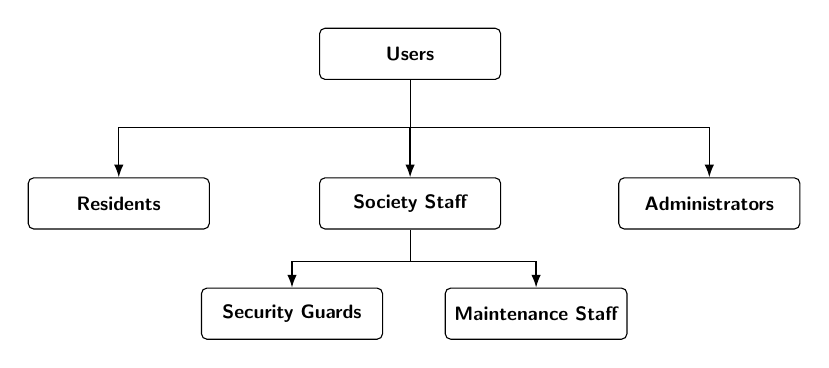
\begin{tikzpicture}[x=1cm,y=1cm]
\node[ubox] (u) at (0,0) {\bfseries Users};
\node[ubox] (r) at (-3.7,-1.9) {\bfseries Residents};
\node[ubox] (s) at (0,-1.9) {\bfseries Society Staff};
\node[ubox] (a) at (3.8,-1.9) {\bfseries Administrators};
\node[ubox] (sg) at (-1.5,-3.3) {\bfseries Security Guards};
\node[ubox] (m) at (1.6,-3.3) {\bfseries Maintenance Staff};
\draw (u.south) -- ++(0,-0.6) coordinate (bus1);
\draw[arr] (bus1) -- (s.north);
\draw (r.north |- bus1) -- (a.north |- bus1);
\draw[arr] (r.north |- bus1) -- (r.north);
\draw[arr] (a.north |- bus1) -- (a.north);
\draw (s.south) -- ++(0,-0.4) coordinate (bus2);
\draw (sg.north |- bus2) -- (m.north |- bus2);
\draw[arr] (sg.north |- bus2) -- (sg.north);
\draw[arr] (m.north |- bus2) -- (m.north);
\end{tikzpicture}
\caption{type of users}
\end{figure}

\subsection{Product Functions}
``GATED: Apartment Tracker'' stores all the data of the society, such as residents, apartments, complaints, visitors, notices and amenity bookings. Before using the main functions of the software, users have to be registered and authenticated. The system tracks comprehensive profile data and relational links across 17 structured database entities.

\begin{figure}[H]
\centering
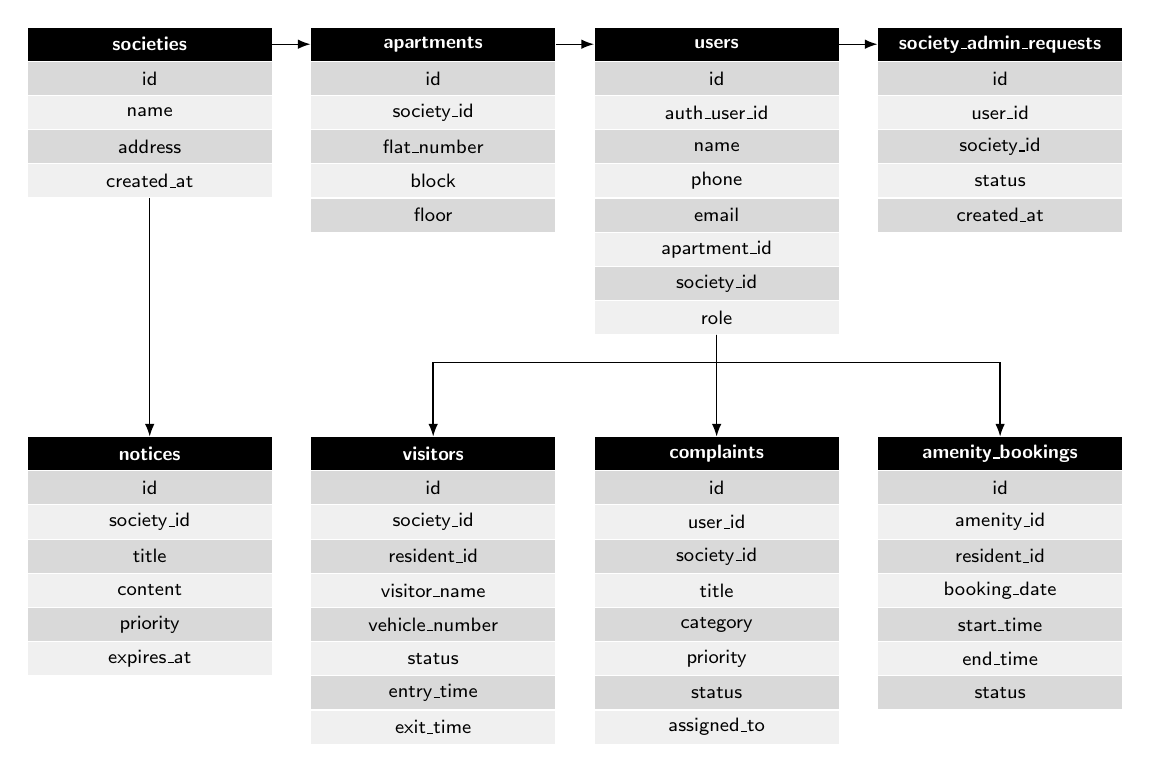
\begin{tikzpicture}[x=1cm,y=1cm]
\dbtable{soc}{1.55,0}{societies}{id,name,address,created\_at}{3.1cm}
\dbtable{apt}{5.15,0}{apartments}{id,society\_id,flat\_number,block,floor}{3.1cm}
\dbtable{usr}{8.75,0}{users}{id,auth\_user\_id,name,phone,email,apartment\_id,society\_id,role}{3.1cm}
\dbtable{sar}{12.35,0}{society\_admin\_requests}{id,user\_id,society\_id,status,created\_at}{3.1cm}

\dbtable{ntc}{1.55,-5.2}{notices}{id,society\_id,title,content,priority,expires\_at}{3.1cm}
\dbtable{vis}{5.15,-5.2}{visitors}{id,society\_id,resident\_id,visitor\_name,vehicle\_number,status,entry\_time,exit\_time}{3.1cm}
\dbtable{cmp}{8.75,-5.2}{complaints}{id,user\_id,society\_id,title,category,priority,status,assigned\_to}{3.1cm}
\dbtable{amb}{12.35,-5.2}{amenity\_bookings}{id,amenity\_id,resident\_id,booking\_date,start\_time,end\_time,status}{3.1cm}

\draw[arr] (soc.east) -- (apt.west);
\draw[arr] (apt.east) -- (usr.west);
\draw[arr] (usr.east) -- (sar.west);
\draw[arr] (soc-4.south) -- (ntc.north);
\draw[arr] (usr-8.south) -- (cmp.north);
\draw[arr] (usr-8.south) -- ++(0,-0.35) -| (vis.north);
\draw[arr] (usr-8.south) -- ++(0,-0.35) -| (amb.north);
\end{tikzpicture}
\caption{Data Flow Diagram}
\end{figure}

The main entities and their attributes are as follows.
\begin{itemize}
\item \textbf{User:} \code{id}, \code{auth\_user\_id}, \code{name}, \code{phone}, \code{email}, \code{apartment\_id}, \code{society\_id}, \code{role}, \code{created\_at}.
\item \textbf{Apartment:} \code{id}, \code{society\_id}, \code{flat\_number}, \code{block}, \code{floor}, \code{created\_at}.
\item \textbf{Complaint and Maintenance Request:} \code{id}, \code{user\_id}, \code{society\_id}, \code{title}, \code{description}, \code{category} (Electrical, Plumbing, HVAC, Security, Other), \code{priority} (low, medium, high), \code{status} (pending, assigned, in\_progress, resolved), \code{assigned\_to}, \code{resolution\_note}, \code{created\_at}, \code{updated\_at}.
\item \textbf{Visitor:} \code{id}, \code{society\_id}, \code{resident\_id}, \code{visitor\_name}, \code{vehicle\_number}, \code{status}, \code{entry\_time}, \code{exit\_time}.
\item \textbf{Notice:} \code{title}, \code{content}, \code{priority}, \code{expires\_at}.
\item \textbf{Amenity Booking:} \code{amenity\_id}, \code{resident\_id}, \code{booking\_date}, \code{start\_time}, \code{end\_time}, \code{status}.
\end{itemize}

\subsection{Operating Environment}
\textbf{Client platforms:}
\begin{itemize}
\item Mobile: Android (Android 9.0 and above) and iOS (iOS 14.0 and above) via React Native / Expo runtime.
\item Web: modern HTML5 browsers (Chrome, Safari, Firefox, Edge) via Expo Web.
\end{itemize}
\textbf{Backend and cloud infrastructure:}
\begin{itemize}
\item Supabase Cloud with PostgreSQL database engine.
\item Supabase Auth (JWT token-based authorization and session tracking).
\item PostgreSQL Row Level Security (RLS) policies enforcing multi-tenant isolation.
\end{itemize}

\subsection{Design}
Resident activities have 3 steps -
\begin{itemize}
\item Onboarding and Registration
\item Service Request Creation
\item Resident Dashboard Tracking
\end{itemize}

The resident first inputs basic credentials, chooses the society from the active society list, specifies the apartment (flat number, block) and completes authentication. After that the resident submits a complaint or maintenance request, selecting category, setting priority and entering details. Then the resident can enter the dashboard.\\
Every resident dashboard contains his/her personal information, complaints with real-time progress, notices and amenity bookings.\\
Notice will contain all the announcements of the society.

\begin{figure}[H]
\centering
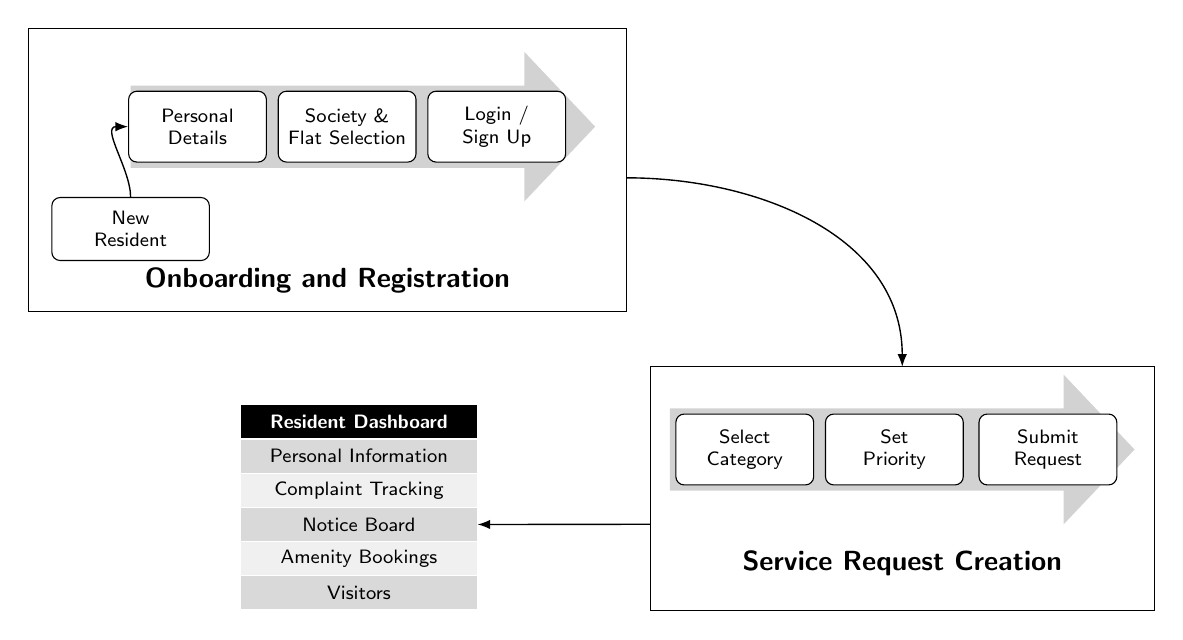
\begin{tikzpicture}[x=1cm,y=1cm]
% Box 1: registration
\draw (0,0) rectangle (7.6,-3.6);
\bigarrow{1.3}{-1.25}{5.9}{0.95}
\node[stp] (s1) at (2.15,-1.25) {Personal\\Details};
\node[stp] (s2) at (4.05,-1.25) {Society \&\\Flat Selection};
\node[stp] (s3) at (5.95,-1.25) {Login /\\Sign Up};
\node[stp,minimum width=2cm,minimum height=0.8cm] (nr) at (1.3,-2.55) {New\\Resident};
\draw[arr] (nr.north) to[out=90,in=180] (s1.west);
\node[font=\sffamily\bfseries\normalsize] at (3.8,-3.2) {Onboarding and Registration};

% Box 2: service request
\draw (7.9,-4.3) rectangle (14.3,-7.4);
\bigarrow{8.15}{-5.35}{5.9}{0.95}
\node[stp] (r1) at (9.1,-5.35) {Select\\Category};
\node[stp] (r2) at (11.0,-5.35) {Set\\Priority};
\node[stp] (r3) at (12.95,-5.35) {Submit\\Request};
\node[font=\sffamily\bfseries\normalsize] at (11.1,-6.8) {Service Request Creation};

\draw[arr] (7.6,-1.9) to[out=0,in=90] (11.1,-4.3);

% Dashboard
\begin{scope}[font=\sffamily\scriptsize]
\node[thead,minimum width=3cm] (dh) at (4.2,-5.0) {Resident Dashboard};
\node[trow,minimum width=3cm,fill=gray!30,below=0pt of dh.south] (d1) {Personal Information};
\node[trow,minimum width=3cm,fill=gray!12,below=0pt of d1.south] (d2) {Complaint Tracking};
\node[trow,minimum width=3cm,fill=gray!30,below=0pt of d2.south] (d3) {Notice Board};
\node[trow,minimum width=3cm,fill=gray!12,below=0pt of d3.south] (d4) {Amenity Bookings};
\node[trow,minimum width=3cm,fill=gray!30,below=0pt of d4.south] (d5) {Visitors};
\end{scope}
\draw[arr] (7.9,-6.3) to[out=180,in=0] (d3.east);
\end{tikzpicture}
\caption{Resident Activities}
\end{figure}

Administrator activities have 2 steps -
\begin{itemize}
\item Society Administrator
\item Maintenance Staff
\end{itemize}

Society Administrator can verify pending admin signups (grant or reject access), review complaints, assign them to specific maintenance staff using employee identifiers and publish notices.\\
Maintenance Staff views only the work orders assigned to him/her, executes the field repairs and updates the task status up to resolution.

\begin{figure}[H]
\centering
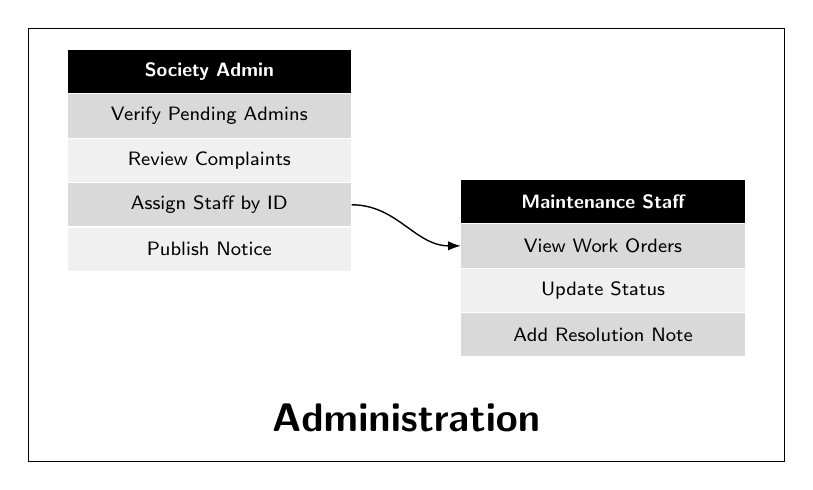
\begin{tikzpicture}[x=1cm,y=1cm]
\draw (0,0) rectangle (9.6,-5.5);
\begin{scope}[font=\sffamily\small]
\node[thead,minimum width=3.6cm,minimum height=0.55cm] (ah) at (2.3,-0.55) {Society Admin};
\node[trow,minimum width=3.6cm,minimum height=0.55cm,fill=gray!30,below=0pt of ah.south] (a1) {Verify Pending Admins};
\node[trow,minimum width=3.6cm,minimum height=0.55cm,fill=gray!12,below=0pt of a1.south] (a2) {Review Complaints};
\node[trow,minimum width=3.6cm,minimum height=0.55cm,fill=gray!30,below=0pt of a2.south] (a3) {Assign Staff by ID};
\node[trow,minimum width=3.6cm,minimum height=0.55cm,fill=gray!12,below=0pt of a3.south] (a4) {Publish Notice};

\node[thead,minimum width=3.6cm,minimum height=0.55cm] (mh) at (7.3,-2.2) {Maintenance Staff};
\node[trow,minimum width=3.6cm,minimum height=0.55cm,fill=gray!30,below=0pt of mh.south] (m1) {View Work Orders};
\node[trow,minimum width=3.6cm,minimum height=0.55cm,fill=gray!12,below=0pt of m1.south] (m2) {Update Status};
\node[trow,minimum width=3.6cm,minimum height=0.55cm,fill=gray!30,below=0pt of m2.south] (m3) {Add Resolution Note};
\end{scope}
\draw[arr] (a3.east) to[out=0,in=180] (m1.west);
\node[font=\sffamily\bfseries\Large] at (4.8,-4.95) {Administration};
\end{tikzpicture}
\caption{Administrator Activities}
\end{figure}

Security staff has only one activity group -
\begin{itemize}
\item Visitor and Gate Logging
\end{itemize}

Security staff verifies the visitor information, registers visitor names and vehicle plates, and records the entry and departure timestamps.

\begin{figure}[H]
\centering
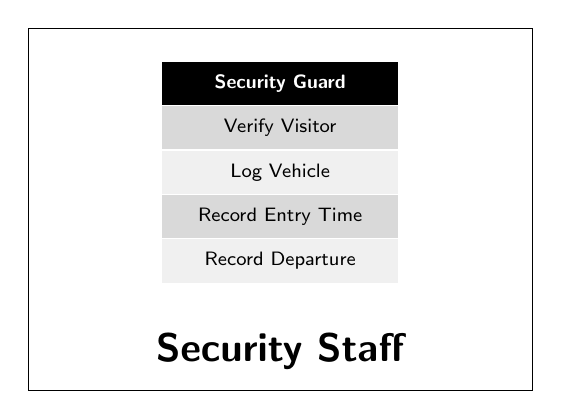
\begin{tikzpicture}[x=1cm,y=1cm]
\draw (0,0) rectangle (6.4,-4.6);
\begin{scope}[font=\sffamily\small]
\node[thead,minimum width=3.0cm,minimum height=0.55cm] (sh) at (3.2,-0.7) {Security Guard};
\node[trow,minimum width=3.0cm,minimum height=0.55cm,fill=gray!30,below=0pt of sh.south] (s1) {Verify Visitor};
\node[trow,minimum width=3.0cm,minimum height=0.55cm,fill=gray!12,below=0pt of s1.south] (s2) {Log Vehicle};
\node[trow,minimum width=3.0cm,minimum height=0.55cm,fill=gray!30,below=0pt of s2.south] (s3) {Record Entry Time};
\node[trow,minimum width=3.0cm,minimum height=0.55cm,fill=gray!12,below=0pt of s3.south] (s4) {Record Departure};
\end{scope}
\node[font=\sffamily\bfseries\Large] at (3.2,-4.1) {Security Staff};
\end{tikzpicture}
\caption{Staff Activities}
\end{figure}

% ====================== 3 SYSTEM FEATURES ======================
\newpage
\section{System Features}
``GATED: Apartment Tracker'' is a society management software. So the main part of this product is to log, delegate and track the issues and the gate activities of the society.

\subsection{Description and Priority}
``GATED: Apartment Tracker'' has features that are main and also some are sub. But all the features are necessary for this software.

The features with priority up to down -
\begin{enumerate}
\item \textbf{User Authentication and Role-Based Access Control} (High / Critical): Secure signup, login, session retention and automated redirection to role-specific dashboards.
\item \textbf{Complaint and Maintenance Lifecycle Management} (High / Critical): Full lifecycle support for resident issues: submission, administrator review, maintenance delegation and status progression (Pending $\rightarrow$ Assigned $\rightarrow$ In Progress $\rightarrow$ Resolved).
\item \textbf{Society Administration and Staff Assignment} (High): Administrative controls for assigning tickets to employees by ID and managing admin account approvals.
\item \textbf{Security Portal and Visitor Logging} (Medium-High): Logging of guest names, vehicle numbers and physical gate entry/exit timestamps.
\item \textbf{Notice Board Broadcasts} (Medium): Publication of society-wide notices and urgent announcements.
\item \textbf{Amenity Reservation System} (Medium): Booking of clubhouse, tennis courts and party halls with slot conflict prevention.
\item \textbf{Emergency Contacts and Billing History} (Low-Medium): Emergency SOS access and historical society maintenance fee tracking.
\end{enumerate}

\subsection{Functional Requirements}
\textbf{FR-1: User Authentication and Role Verification}
\begin{itemize}
\item \textbf{FR-1.1:} The system shall allow users to register with name, phone number, email address and password (minimum 6 characters).
\item \textbf{FR-1.2:} The system shall require users to choose one of four predefined roles: Resident, Society Admin, Security Staff or Maintenance Staff.
\item \textbf{FR-1.3:} The system shall restrict Resident onboarding to valid apartments belonging to the chosen society.
\item \textbf{FR-1.4:} The system shall place all newly registered Society Admin accounts into a \code{pending} state until approved by an existing admin.
\end{itemize}

\textbf{FR-2: Resident Dashboard and Request Creation}
\begin{itemize}
\item \textbf{FR-2.1:} The system shall display the logged-in resident's name, society, flat number, active complaints, notices and bookings.
\item \textbf{FR-2.2:} The system shall provide a request creation form supporting both Complaints and Maintenance Requests.
\item \textbf{FR-2.3:} The form shall require a title, category (Electrical, Plumbing, HVAC, Security, Other), priority (low, medium, high) and description.
\end{itemize}

\textbf{FR-3: Administrator Complaint Assignment}
\begin{itemize}
\item \textbf{FR-3.1:} The admin dashboard shall list all unresolved complaints submitted within the administrator's society.
\item \textbf{FR-3.2:} The system shall allow administrators to assign a complaint to an active maintenance staff member by entering their employee ID.
\item \textbf{FR-3.3:} Upon successful assignment, the ticket status shall automatically transition to \code{assigned}.
\end{itemize}

\textbf{FR-4: Maintenance Staff Work Execution}
\begin{itemize}
\item \textbf{FR-4.1:} Maintenance staff shall only be presented with complaints and service requests assigned to their specific user ID.
\item \textbf{FR-4.2:} Staff shall be able to update ticket statuses through \code{in\_progress} to \code{resolved}.
\end{itemize}

\textbf{FR-5: Visitor Verification and Gate Logging}
\begin{itemize}
\item \textbf{FR-5.1:} Security personnel shall be able to create visitor entry logs capturing visitor name, host resident ID, vehicle registration and entry timestamp.
\item \textbf{FR-5.2:} Security personnel shall be able to record exit timestamps upon visitor departure.
\end{itemize}

\textbf{FR-6: Technology Stack Specification}\\
The ``GATED: Apartment Tracker'' application is being built with React Native, Expo, TypeScript and Supabase.\\
Front-End - React Native (0.86), Expo SDK (57), Expo Router, TypeScript, React 19.\\
Styling - Custom theme stylesheet (\code{\#91441F} brown, \code{\#FFF9F7} background, \code{\#FFF0EB} peach).\\
Back-End / Services - Supabase Cloud, Supabase Auth.\\
Database - PostgreSQL 15+.

% ====================== 4 NONFUNCTIONAL ======================
\newpage
\section{Other Nonfunctional Requirements}
\subsection{Performance Requirements}
\begin{itemize}
\item \textbf{Response Time:} Database queries and API calls via the Supabase client shall return within 500 ms under standard mobile network conditions (4G/5G/Wi-Fi).
\item \textbf{Startup Time:} The mobile client shall authenticate session tokens and display the appropriate dashboard within 2 seconds.
\item \textbf{Concurrency:} The database schema shall support concurrent operations across multiple societies without deadlocks or data cross-contamination.
\end{itemize}

\subsection{Security Requirements}
\begin{itemize}
\item \textbf{Authentication and Encryption:} User passwords must be encrypted using strong cryptographic hashing algorithms (bcrypt/Argon2) handled via Supabase Auth.
\item \textbf{Session Tokens:} Client sessions shall use secure JWT bearer tokens stored in secure asynchronous device storage.
\item \textbf{Data Isolation (Row Level Security):} PostgreSQL Row Level Security (RLS) policies must guarantee that residents can only view and mutate their own records, and administrators can only manage records within their own society.
\item \textbf{Privilege Separation:} Users attempting to access dashboards outside their assigned role must be blocked and redirected to the login screen.
\end{itemize}

\subsection{Software Quality Attributes}
\begin{itemize}
\item \textbf{Maintainability:} The codebase adheres to strict TypeScript typings, a modular React component architecture (separated into \code{admin}, \code{resident} and \code{ui} packages) and clean file-based routing.
\item \textbf{Usability:} The interface uses high-contrast typography, recognizable SF Symbols / Material icons and clear visual state badges (Pending, Assigned, Resolved).
\item \textbf{Reliability:} All database foreign key constraints are enforced to ensure that orphan records cannot exist if an apartment, society or user is deleted.
\end{itemize}

\subsection{Business Rules}
\begin{itemize}
\item \textbf{BR-1:} Every resident must be associated with exactly one society and one apartment unit.
\item \textbf{BR-2:} Maintenance tickets can only be assigned to maintenance staff registered within the exact same society as the complaint.
\item \textbf{BR-3:} Society admin requests remain non-operational in \code{pending} status until an approved admin explicitly confirms the request.
\item \textbf{BR-4:} Double booking of any society amenity for overlapping time intervals is prohibited.
\end{itemize}

% ====================== 5 OTHER REQUIREMENTS ======================
\newpage
\section{Other Requirements}
``GATED: Apartment Tracker'' needs maintenance as it is designed for long-term, multi-semester evolution. It will need refactoring and further the requirements can be changed as the field is changing frequently. Ongoing maintenance includes:
\begin{itemize}
\item Periodic database migrations to update relational schemas as new society amenities and workflows are added.
\item Periodic dependency maintenance to keep compatibility with new versions of the Expo SDK and React Native runtime.
\end{itemize}

The platform architecture is designed to support the following planned enhancements:
\begin{enumerate}
\item \textbf{Dynamic QR Visitor Passes:} Residents generate time-limited QR codes that security guards scan at the gate for contactless verification.
\item \textbf{Push Notifications:} Instant notifications dispatched to residents when visitors arrive or when a complaint status changes.
\item \textbf{Integrated Online Payments:} Payment gateway integration (Razorpay/Stripe) for society maintenance fees and amenity booking security deposits.
\item \textbf{Emergency SOS System:} One-tap emergency broadcast alerting society guards and neighbors in urgent situations.
\end{enumerate}

\end{document}